\documentclass[../main.tex]{subfiles}

\begin{document}
\subsection{Introduction}
\subsubsection{Complex Number.} Complex number may be written in the rectangular form or polar form
\begin{align*}
    z=x+i y=re^{i\theta}=r(\cos\theta+i\sin\theta)
\end{align*}
The quantity $r$ is called the modulus or absolute value of $z$, and $\theta$ is called the angle of $z$ (or the phase, or the argument, or the amplitude of $z$). In symbols
\begin{align*}
    \mathrm{Re}\; z&=x&&    |z|=\text{mod } z=r=\sqrt{x^2+y^2}=\sqrt{z\bar{z}}\\
    \mathrm{Im}\; z&=y\;\textrm{(not $iy$)}&&\text{angle of } z=\theta
\end{align*}
The values of $\theta$ should be found from a diagram rather than a formula, although we do sometimes write $\theta = \arctan(y/x)$. Word of caution however, the domain of $\arctan x$ is restricted to $(-\pi/2, \pi/2)$. here's another useful (?) operator formula
\begin{align*}
    \mathrm{Re}\; z&=\frac{z+\bar{z}}{z}\\
    \mathrm{Im}\; z&=\frac{z-\bar{z}}{zi}
\end{align*}

\subsubsection{Conjugate.} Complex numbers come in conjugate pairs; for such pairs are mirror images of each other with the x axis as the mirror. If we write $z = r(\cos \theta + i \sin \theta)$, then
\begin{align*}
    \bar{z}=re^{-i\theta}=r(\cos\theta-i\sin\theta)
\end{align*}

\subsection{Euler's Formula.} Using series expansion, we write $e^{i\theta}$, where $\theta$ is real
\begin{align*}
    e^{i\theta}&=1+i\theta+\frac{(i\theta)^2}{2!}+\frac{(i\theta)^3}{3!}+\frac{(i\theta)^4}{4!}+\frac{(i\theta)^5}{5!}\dots\\
    &=1+i\theta- \frac{\theta^2}{2!}-i\frac{\theta^3}{3!}+\frac{\theta^4}{4!}+i\frac{\theta^5}{5!}\dots\\
    &=1- \frac{\theta^2}{2!}+\frac{\theta^4}{4!}+\dots+i\biggl(+\theta-\frac{\theta^3}{3!}+\frac{\theta^5}{5!}\dots\biggr)
\end{align*}
We then have the very useful result known as Euler's formula
\begin{align*}
    e^{i\theta}=\cos\theta+i\sin\theta\\
\end{align*}

Remembering that any complex number can be written in the form $re^{i\theta}$, we get
\begin{equation*}
    z_1\times z_2=r_1r_2e^{i(\theta_1+\theta_2)}\quad\text{and}\quad z_1\div z_2=\frac{r_1}{r_2}e^{i(\theta_1-\theta_2)}
\end{equation*}

Using the rules for multiplication and division of complex numbers, we have
\begin{equation*}
    z^n = (re^{i\theta})^n = r^ne^{in\theta}
\end{equation*}
for any integral $n$.  The case $r = 1$, the equation becomes DeMoivre's theorem:
\begin{equation*}
    e^{in\theta}=\cos n\theta + i \sin n\theta
\end{equation*}

\subsection{Function of Complex Number}. We define $e^z$ by the power series
\begin{equation*}
    e^z=\sum_{0}^{\infty}\frac{z}{n!}=1+z+\frac{z^2}{2!}+\frac{z^3}{3!}+\dots
\end{equation*}
then we can write 
\begin{equation*}
    e^z=e^{x+iy}  = e^x(\cos y + i \sin y).
\end{equation*}

We then write Euler's formula, in $\theta$ and $-\theta$
\begin{align*}
    e^{i\theta}&=\cos\theta+i\sin\theta\\
    e^{-i\theta}&=\cos\theta-i\sin\theta
\end{align*}
These two equations can be solved for $\sin\theta$ and $\cos\theta$
\begin{align*}
    \sin \theta&=\frac{e^{i\theta}-e^{-i\theta}}{2i}\\
    \cos \theta&=\frac{e^{i\theta}+e^{-i\theta}}{2}
\end{align*}
These formulas are useful in evaluating integrals since products of exponentials are 
easier to integrate than products of sines and cosines. 

We could also define $\sin z$ and $\cos z$ for complex $z$ by their power series as we did for $e^z$, however it is simpler to use the complex equations we just obtained to define  $\sin z$ and $\cos z$
\begin{align*}
    \sin z&=\frac{e^{iz}-e^{-iz}}{2i}\\
    \cos z&=\frac{e^{iz}+e^{-iz}}{2}
\end{align*}
The rest of the trigonometric functions of $z$ are defined in the usual way in terms of these; for example, $\tan z = \sin z/ \cos z$

\subsection{Hyperbolic Function}

Hyperbolic sine (abbreviated sinh) and the hyperbolic cosine (abbreviated cosh) is defined from pure imaginary, that is, $ z = iy$. Their definitions for all $z$ are
\begin{align*}
    \sinh z&=\frac{e^{z}-e^{-z}}{2}\\
    \cosh z&=\frac{e^{z}+e^{z}}{2}
\end{align*}
As before, the other hyperbolic functions are named and defined in a similar way to parallel the trigonometric functions. 

We can write 
\begin{align*}
    \sin iy &= i \sinh y\\
    \cos iy&=\cosh y
\end{align*}
Then we see that the hyperbolic functions of $y$ are (except for one $i$ factor) the trigonometric functions of $iy$.

The functions $\sin t, \cos t$, and the rest of the gang are called “circular functions” and the functions $\sinh t, \cosh t,$ etc. are called “hyperbolic functions” because $ x = \cos t, y = \sin t,$ satisfy the equation of a circle $x^2 + y^2 = 1$, while $x = \cosh t,  y = \sinh t,$ satisfy the equation of a hyperbola $x^2 - y^2 = 1$.

\subsection{Logarithm}
If 
\begin{equation*}
    z=e^w
\end{equation*}
then by definition
\begin{equation*}
    w=\ln z
\end{equation*}
We can write the law of exponents, as
\begin{equation*}
    z_1z_2 = e^{w_1+w_2}
\end{equation*}
Taking logarithms of this equation, we get
\begin{equation*}
   \ln z_1z_2 = {w_1+w_2}=\ln z_1+\ln z_2
\end{equation*}
This is the familiar law for the logarithm of a product, justified now for complex numbers. We can then find the real and imaginary parts of the logarithm of a complex number from the equation
\begin{equation*}
    \ln z = ln(re^{i\theta})=\ln r+\ln e^{i\theta}
\end{equation*}
thus
\begin{align*}
    \ln z = \ln r + i\theta= \ln r + i(\theta+2n\pi)
\end{align*}
Since $\theta$ has an infinite number of values (all differing by multiples of $2\pi$), a complex number has infinitely many logarithms, differing from each other by multiples of $2\pi i$.

\subsubsection{Complex Power.} By definition, for complex $a$ and $b$ ($a = e$),
\begin{equation*}
    a^b=e^{b\ln a}
\end{equation*}

\subsection{Analytic Function}
\subsubsection{Introduction to Complex Function.} In general, we write
\begin{equation*}
    f(z) = f(x + iy) = u(x, y) + iv(x, y)
\end{equation*}
where it is understood that $u$ and $v$ are real functions of the real variables x and y. 

Recall that functions are customarily single-valued. Does this mean that we cannot define a function by a formula such as $\ln z$? For each $z$, $\ln z$ has an infinite set of values. But if $\theta$ is allowed a range of only $2\pi$ , then $\ln z$ has one value for each $z$ and this single-valued function is 
called a branch of $\ln z$. Thus in using formulas, we always discuss a single branch at a time so that we have a single-valued function. As a matter of terminology, however, you should know that the 
whole collection of branches is sometimes called a “multiple-valued function.”

\subsubsection{Definition.} A function $f(z)$ is analytic--or regular or holomorphic or monogenic--in a region--region must be two dimensional, isolated points and curves are not regions--of the complex plane if it has a unique derivative at every point of the region. 

 The derivative of $f(z)$ is defined by the equation
 \begin{equation*}
    f'(z)=\frac{df}{dz}=\lim_{\Delta z\rightarrow 0}\frac{\Delta f}{\Delta z}=\lim_{\Delta z\rightarrow 0} \frac{f(z + \Delta z) - f(z)}{\Delta x + i\Delta y}
 \end{equation*}

The statement “$f(z)$ is analytic at a point $z = a$” means that $f(z)$ has a derivative at every point inside some small circle about $z = a$. When we say that $f(x)$ has a derivative at $x = x_0$, we mean that these two values are equal. When we say that $f(z)$ has a derivative at $z = z_0$, we mean that $f'(z)$ has the same value no matter how we approach $z_0$. 

\subsection{Theorems}
\subsubsection{Theorem I: Cauchy-Riemann conditions.} If $f(z) = u(x, y) + iv(x, y)$ is analytic in a 
region, then in that region
\begin{equation*}
    \frac{\partial u}{\partial x}=\frac{\partial v}{\partial y}
    \qquad\text{and}\qquad 
    \frac{\partial v}{\partial x}=-\frac{\partial u}{\partial y}
\end{equation*}

\emph{Proof}. Remembering that $f (z)= f (x + iy)$, we use the rules of partial differentiation 
\begin{equation*}
    \frac{\partial f}{\partial x}=\frac{df}{dz}\frac{\partial z}{\partial x}=\frac{df}{dz}
\end{equation*}
and
\begin{equation*}
    \frac{\partial f}{\partial y}=\frac{df}{dz}\frac{\partial z}{\partial y}=i\frac{df}{dz}
\end{equation*}
Since $f = u(x, y) + iv(x, y)$, we also have
\begin{equation*}
    \frac{\partial f}{\partial x}=\frac{\partial u}{\partial x}+i \frac{\partial v}{\partial x}
\end{equation*}
and
\begin{equation*}
    \frac{\partial f}{\partial y}=\frac{\partial u}{\partial y}+i \frac{\partial v}{\partial y}
\end{equation*}
Combining them we have
\begin{equation*}
    \frac{df}{dz}=\frac{\partial u}{\partial x}+i \frac{\partial v}{\partial x}
\end{equation*}
and
\begin{equation*}
    \frac{df}{dz}=\frac{1}{i}\biggl(\frac{\partial u}{\partial y}+i \frac{\partial v}{\partial y}\biggr) =\frac{\partial v}{\partial y}-i \frac{\partial u}{\partial y}
\end{equation*}

Since we assumed that $df /dz$ exists and is unique (this is what analytic means), these two expressions for $df /dz$ must be equal. Taking real and imaginary parts, we get the Cauchy-Riemann equations. $\quad \blacksquare$

\subsubsection{Theorem II.} If $u(x, y)$ and $v(x, y)$ and their partial derivatives with respect to $x$ and $y$ are continuous and satisfy the Cauchy-Riemann conditions in a region, then $f(z)$ is analytic at all points inside the region--not necessarily on the boundary.

\emph{Proof (?).} Although we shall not prove this, we can make it plausible by showing that it is true when we approach $z_0$ along any straight line. Assuming that we approach $z_0$ along a straight line of slope $m$, we will show that $df /dz$ does not depend on $m$ if $u$ and $v$ satisfy Cauchy-Riemann conditions. The equation of the straight line of slope $m$ through the point $z_0 = x_0 + iy_0$ is
\begin{equation*}
    y - y_0 = m(x - x_0)
\end{equation*}
and along this line we have $dy/dx = m$. Then we find
\begin{align*}
    \frac{df}{dz}&=\frac{du+i\;dv}{dx+i\;dy}\\
    &=\frac{\dfrac{\partial u}{\partial x}dx+\dfrac{\partial u}{\partial y}dy+i\biggl(\dfrac{\partial v}{\partial x}dx+\dfrac{\partial v}{\partial y}dy\biggr)}{dx+i\;dy}\\
    &=\frac{\dfrac{\partial u}{\partial x}+\dfrac{\partial u}{\partial y}m+i\biggl(\dfrac{\partial v}{\partial x}+\dfrac{\partial v}{\partial y}m\biggr)}{1+i\;m}
\end{align*}
Using the Cauchy-Riemann equations, we get
\begin{align*}
    \frac{df}{dz}&=\frac{\dfrac{\partial u}{\partial x}-\dfrac{\partial v}{\partial x}m+i\biggl(\dfrac{\partial v}{\partial x}+\dfrac{\partial u}{\partial x}m\biggr)}{1+i\;m}\\
    &=\frac{\dfrac{\partial u}{\partial x}(1+im)+i\dfrac{\partial v}{\partial y}(1+im)}{1+i\;m}\\
    &=\frac{\partial u}{\partial x}+i\frac{\partial v}{\partial y}
\end{align*}
Thus $df /dz$ has the same value for approach along any straight line. The theorem states that it also has the same value for approach along any curve.

\subsubsection{Theorem III.} If $f(z)$ is analytic in a region $R$, then it has derivatives of all orders at points inside the region and can be expanded in a Taylor series about any point $z_0$ inside the region. The power series converges inside the circle about $z_0$ that extends to the nearest singular point $C$.
\begin{figure*}[h]
    \centering
    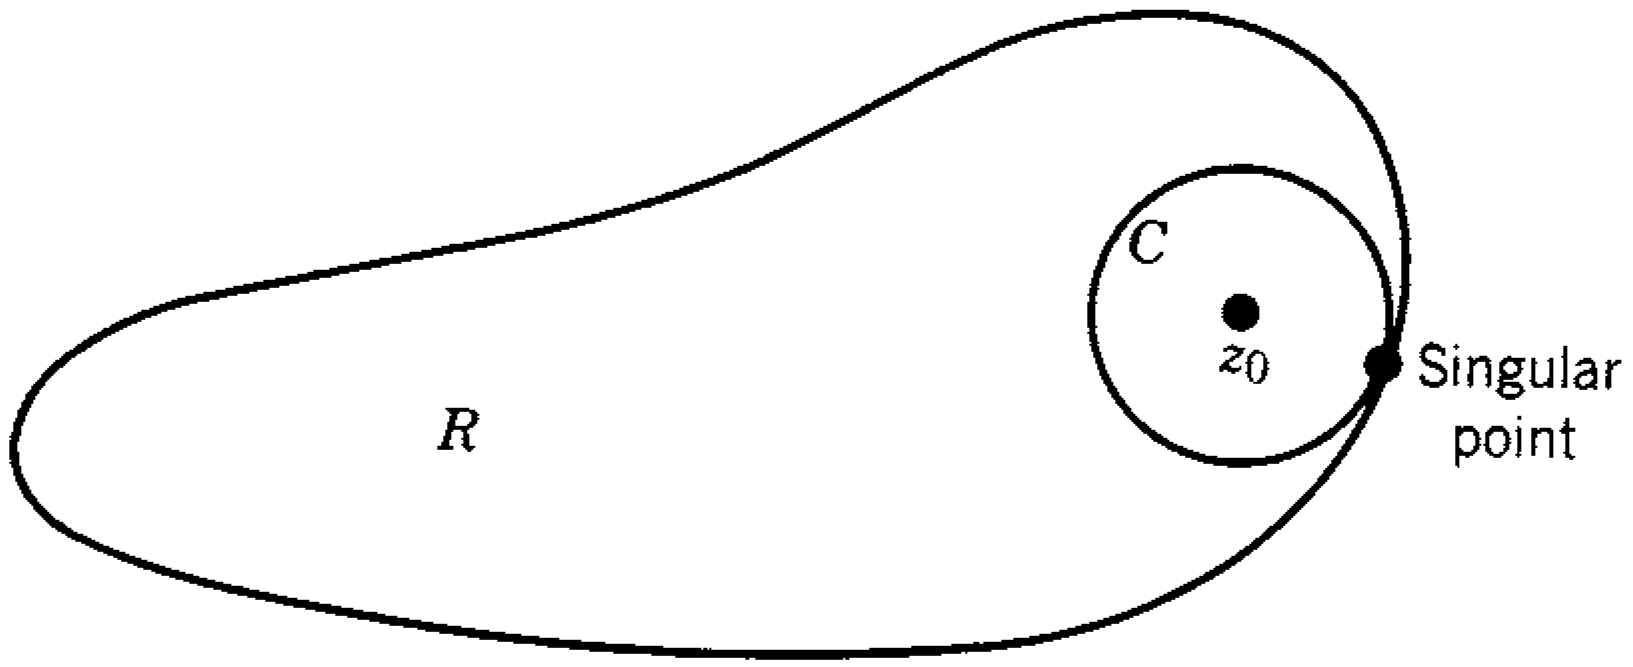
\includegraphics[width=0.5\textwidth]{../Rss/Com/Theorem3.png}
\end{figure*}

\emph{No proof.} Some definitions are in order. A regular point of $f (z)$ is a point at which $f (z)$ is analytic. A singular point or singularity of $f (z)$ is a point at which $f (z)$ is not analytic. It is called an isolated singular point if $f (z)$ is analytic everywhere else inside some small circle about the singular point.

\subsubsection{Theorem IV.} Part 1: if $f(z) = u +iv$ is analytic in a region, then $u$ and $v$ satisfy Laplace's equation in the region--that is, $u$ and $v$ are harmonic functions. 

Part 2: any function $u$--or $v$--satisfying Laplace's equation in a simply-connected region, is the real or imaginary part of an analytic function $f(z)$.

\emph{No proof.} Thus we can find solutions of Laplace's equation simply by taking the real or imaginary parts of an analytic function of $z$. It is also often possible, starting with a simple function which satisfies Laplace's equation, to find the explicit function $f (z)$ of which it is, say, the real part.

\subsubsection{Theorem V: Cauchy's theorem.} Let $C$ be a simple--curve which does not cross itself--closed curve with a continuously turning tangent except possibly at a finite number of points--that is, we allow a finite number of corners, but otherwise the curve must be smooth. If $f(z)$ is analytic on and inside $C$, then
\begin{equation*}
    \oint_C f(z) \;dz = 0
\end{equation*}

\emph{Proof}. We shall prove Cauchy's theorem assuming that $f '(z)$ is continuous.
\begin{align*}
    \oint_C f(z) \;dz =\oint_C  (u + iv)(dx + i \;dy)
\end{align*}
or
\begin{equation*}
    \oint_C f(z) \;dz =\oint_C(u \;dx - v\; dy)+i\oint_C (v\; dx + u\; dy)
\end{equation*}
Green’s theorem in the plane says that if $P (x, y)$, $Q(x, y)$, and their partial derivatives are continuous in a simply-connected region $R$, then
\begin{equation*}
    \oint_C P\;dx+Q\;dy=\int_A \biggl(\frac{\partial Q}{\partial x}- \frac{\partial P}{\partial y}\biggr)\;dx\;dy
\end{equation*}
where $C$ is a simple closed curve lying entirely in $R$ and $A$ is area inside $C$. Applying Green's Theorem to the first integral, we get
\begin{equation*}
    \oint_C(u \;dx - v\; dy)=\int_A \biggl(-\frac{\partial v}{\partial x}- \frac{\partial u}{\partial y}\biggr)\;dx\;dy=\int_A \biggl(\frac{\partial u}{\partial x}- \frac{\partial u}{\partial y}\biggr)\;dx\;dy=0
\end{equation*}
where we have used the Cauchy-Riemann. In the same way the second integral in is zero
\begin{equation*}
    i\oint_C (v\; dx + u\; dy)=
    i\int_A \biggl(\frac{\partial u}{\partial x}- \frac{\partial v}{\partial y}\biggr)\;dx\;dy=
    i\int_A \biggl(\frac{\partial v}{\partial y}- \frac{\partial v}{\partial y}\biggr)\;dx\;dy=0
\end{equation*}

\subsubsection{Theorem VI: Cauchy's integral formula.} If $f(z)$ is analytic on and inside a simple closed curve $C$, the value of $f(z)$ at a point $z = a$ inside $C$ is given by the following contour integral along $C$:
\begin{equation*}
    f(a)=\frac{1}{2\pi i}\oint \frac{f(z)}{z-a}\;dz
\end{equation*}
\begin{figure*}[h]
    \centering
    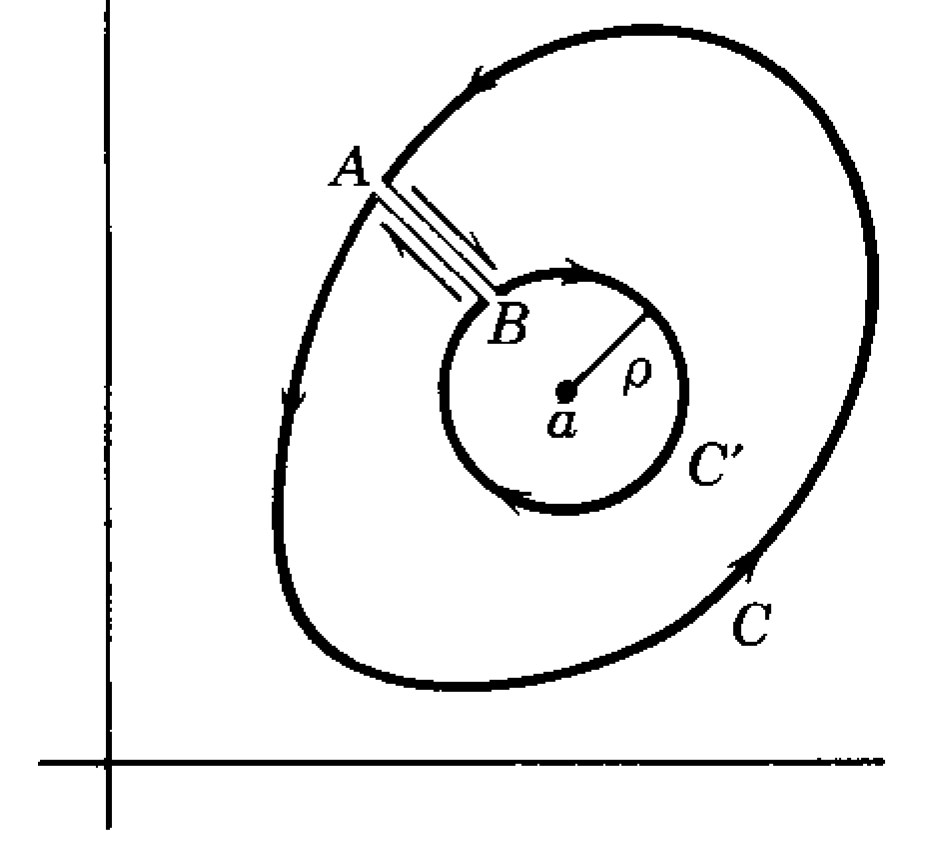
\includegraphics[width=0.5\textwidth]{../Rss/Com/Theo.png}
\end{figure*}

\emph{Proof.} Let a be a fixed point inside the simple closed curve C and consider the function
\begin{equation*}
    \phi(z)=\frac{f(z)}{z-a}
\end{equation*}
where $f(z)$ is analytic on and inside $C$. Let $C'$ be a small circle (inside $C$) with center at a and radius $\rho$. Thus we have 
\begin{equation*}
    \oint_{C\circlearrowleft} \phi(z)\;dz+\oint_{C'\circlearrowright} \phi(z)\;dz=0
\end{equation*}
and
\begin{equation*}
    \oint_{C\circlearrowleft} \phi(z)\;dz=\oint_{C'\circlearrowleft} \phi(z)\;dz
\end{equation*}
where both are counterclockwise. Along the circle $C'$,
\begin{align*}
    z&= a + \rho e^{i\theta}\\
    dz&=\rho i e^{i\theta}\;d\theta
\end{align*}
and the integral becomes
\begin{equation*}
    \oint_{C'\circlearrowleft} \phi(z)\;dz=\int_{0}^{2\pi} \frac{f(z)}{ \rho e^{i\theta}}\;\rho i e^{i\theta}\;d\theta=\int_{0}^{2\pi}f(z)i\;d\theta
\end{equation*}
Since our calculation is valid for any (sufficiently small) value of $\rho$, we shall let
$\rho\rightarrow0$ (that is, $z\rightarrow a$) to simplify the formula
\begin{equation*}
    \oint_{C'\circlearrowleft} \phi(z)\;dz=\int_{0}^{2\pi}f(a)i\;d\theta=2\pi if(a)
\end{equation*}
thus
\begin{equation*}
    f(a)=\frac{1}{2\pi i}\oint \frac{f(z)}{z-a}\;dz \quad \blacksquare
\end{equation*}

\subsubsection{Theorem VII: Laurent's theorem.} Let $C_1$ and $C_2$ be two circles with center at $z_0$. Let $f(z)$ be analytic in the region $R$ between the circles. Then $f(z)$ can be expanded in a series of the form
\begin{equation*}
    f(z) = a_0 + a_1(z - z_0) + a_2(z - z_0)^2+\dots+\frac{b_1}{z-z_0}+\frac{b_2}{(z-z_0)^2}+\dots
\end{equation*}
convergent in $R$. Such a series is called a Laurent series. The $b$ series is called the principal part of the Laurent series.

\emph{Definition.} If all the $b$’s are zero, $f (z)$ is analytic at $z = z_0$, and we call $z_0$ a regular point.

If $b_n \neq 0$, but all the $b$’s after $b_n$ are zero, $f (z)$ is said to have a pole of order $n$ at $z = z_0$. If $n = 1$, we say that $f (z)$ has a simple pole.

If there are an infinite number of $b$’s different from zero, $f (z)$ has an essential singularity at $z = z_0$.

The coefficient $b_1$ of $1/(z - z_0)$ is called the residue of $f (z)$ at $z = z_0$.

\subsection{Residue Theorem}
Suppose we are going to find the value of $\oint  f (z) \;dz$ around a simple closed curve $C$ surrounding an isolated singular point $z_0$ but inclosing no other singularities. Let $f (z)$ be expanded in the Laurent series about $z = z_0$. The integral of the $a$ series 
\begin{equation*}
    \oint_C a_n(z-z0)^n\;dz=0
\end{equation*}
since this pat is analytic. The integral of the $b$ series, we replace the integrals around $C$ by integrals around a circle $C'$ with center at $z_0$ and radius $\rho$
\begin{equation*}
    \oint_{C'} \frac{b_n}{(z-z_0)^n}\;dz=i\int_{0}^{2\pi}b_ne^{i\theta(1-n)}d\theta=\frac{b_n}{1-n}\biggl(e^{2\pi i (1-n)}-1\biggr)=0
\end{equation*}
for all $n>1$. For $n=1$
\begin{equation*}
    \oint_{C'} \frac{b_1}{(z-z_0)}\;dz=ib_1\int_{0}^{2\pi}d\theta=2\pi i b_1
\end{equation*}
Then
\begin{equation*}
    \oint_{C'}  f (z) \;dz=2\pi i b_1
\end{equation*}
since $b_1$ is called the residue of $f (z)$ at $z = z_0$, we can say
\begin{equation*}
    \oint_c  f (z) \;dz=2\pi i \times \text{residue of $f (z)$ at the singular point inside $C$}
\end{equation*}
The only term of the Laurent series which has survived the integration process is the $b_1$ term; you can see the reason for the term “residue.” Thus we have the residue theorem:
\begin{equation*}
    \oint_C  f (z) \;dz=2\pi i\; R(z)
\end{equation*}
where $R(z)$ sum of the residues of $f (z)$ inside $C$.

\subsection{Method of Finding Residue}
\subsubsection{Laurent Series.} If it is easy to write down the Laurent series for $f (z)$ about $z = z_0$ that is valid near $z_0$, then the residue is just the coefficient $b_1$ of the term $1/(z - z0)$. \textbf{Caution}: Be sure you have the expansion about $z = z_0$.

\subsubsection{Simple Pole.} If $f (z)$ has a simple pole at $z = z_0$, we find the residue by multiplying $f (z)$ by $(z - z_0)$ and evaluating the result at $z = z_0$. In general we write
\begin{equation*}
    R(z_0) = \lim_{z\rightarrow z_0} (z - z_0)f (z)\bigg|_{z=z_0}
\end{equation*}
when $z_0$ is a simple pole. If, $f (z)$ can be written as $g(z)/h(z)$, where $g(z)$ is analytic and not zero at $z_0$ and $h(z_0) = 0$, then 
\begin{equation*}
    R(z_0) = \lim_{z\rightarrow z_0} (z - z_0)\frac{g(z)}{h(z)}
    =g(z_0)\lim_{z\rightarrow z_0}\frac{ (z - z_0)}{h(z)}
    =\frac{g(z_0)}{h'(z_0)}
\end{equation*}
In another words
\begin{equation*}
    R(z_0)=\frac{g(z_0)}{h'(z_0)}\begin{cases}
        (z) = g(z)/h(z), \\
        g(z_0) =C\neq 0,\\
        h(z_0) = 0,\\
        h'(z_0) \neq  0
    \end{cases}
\end{equation*}

Perhaps the simplest way--without finding the Laurent series--to find if a function has a simple pole is that if the limit obtained is some constant not $0$ or $\infty$, then $f (z)$ does have a simple pole and the constant is the residue. If the limit is equal to 0, the function is analytic and the residue is 0. If the limit is infinite, the pole is of higher order.

Suppose $f (z)$ is written in the form $g(z)/h(z)$, where $g(z)$ and $h(z)$ are analytic. Then you can think of $g(z)$ and $h(z)$ as power series in $(z - z_0)$. If the denominator has the factor $(z - z_0)$ to one higher power than the numerator, then $f (z)$ has a simple pole at $z_0$. 

\subsubsection{Multiple Poles.} When $f (z)$ has a pole of order $n$, we can use the following
method of finding residues.
\begin{equation*}
    R(z_0)=\frac{1}{(m-1)!}\biggl(\frac{d}{dz}\biggr)^{m-1}\biggl((z-z_0)^mf(z)\biggr)\bigg|_{z=z_0}
\end{equation*}
where $m$ is an integer greater than or equal to the order $n$ of the pole. To compute the derivative quickly, use Leibniz’ rule for differentiating a product
\begin{equation*}
    \biggl(\frac{d}{dx}\biggr)^{n}fg=\sum_{k=0}^n {n \choose k}\biggl(\frac{d}{dx}\biggr)^{n-k} f \biggl(\frac{d}{dx}\biggr)^{k}g
\end{equation*}
where
\begin{equation*}
    {n \choose k}={\frac{n!}{k! (n-k)!}}
\end{equation*}
\end{document}